\chapter{算法介绍}
\section{引言}
本文基本的研究思路是使用数值模拟算法和深度学习算法来研究流变学本构方程建模。本文研究第一部分基于动态时序建模理论和PINN的物理约束理论,构建PI-GRU的预测模型,通过深度学习算法处理数值模拟生成的时变本构关系数据,重点解析循环神经网络在时间序列建模中的特征提取机制,主要涉及的算法模型有循环时间网络类算法模型,本章同时综述了时间序列数据的其他深度学习算法。第二部分引入物理约束的智能建模策略,针对实际流变实验数据构建融合物理信息的混合神经网络模型,重点整合了PINN的微分方程嵌入技术、基于注意力机制驱动的多源特征融合方法,以及结合CVAE的生成式建模策略,实现物理规律约束下的数据-模型双驱动建模。

本章将在此基础上,对研究中所涉及的关键算法进行理论概述,并阐述实验中算法选型的依据,以系统性地综述相关领域的研究进展,为后续研究奠定理论基础。
\section{算法介绍}
\subsection{时间序列数据介绍}
时间序列数据是指一系列时间点上按时间顺序排列的数据点集合。这些数据点通常是连续或定期记录的,反映了某个变量随时间的变化情况。在流变学研究中,时间域的应力应变数据在小应变时满足玻尔兹曼叠加原理,即当前应力状态为之前所有应变历史的线性叠加\cite{boltzmannZurTheorieElastischen1878}。大应变时应力应变数据虽然不满足玻尔兹曼的线性叠加,但是依旧可以表示为过去应变历史的非线性函数叠加。

\subsection{循环神经网络}
\subsubsection{简单RNN}
循环神经网络(Recurrent Neural Network, RNN)是一种专门处理序列数据的神经网络结构,其核心在于利用循环结构捕捉时间或顺序上的依赖关系\cite{elmanFindingStructureTime1990}。RNN的基本结构由输入层、隐藏层和输出层组成(图\ref{rnn_gru illustration}(a))。隐藏层中的神经元不仅接收来自输入层的信号,还接收来自前一时刻隐藏层的信号。这种循环连接使得RNN能够捕获序列中的时间依赖关系。
RNN的数学模型可以通过公式\eqref{eq:rnnht}描述:
\begin{align}
   & \mathbf{h}_t = \sigma(\mathbf{W}_{xh} \mathbf{x}_t + \mathbf{W}_{hh} \mathbf{h}_{t-1} + \mathbf{b}_h) \label{eq:rnnht} \\
   & {\mathbf{o}_t = \mathbf{W}_{ho} \mathbf{h}_t + \mathbf{b}_o} \label{eq:rnnot}
\end{align}
其中$\mathbf{h}_t$ 是时刻 $t$ 的隐藏状态,$\mathbf{x}_t$ 是时刻 $t$ 的输入,$\mathbf{o}_t$ 是时刻 $t$ 的输出,$\mathbf{W}_{xh}$ 是输入到隐藏层的权重矩阵,$\mathbf{W}_{hh}$ 是隐藏层到隐藏层的权重矩阵,$\mathbf{W}_{ho}$ 是隐藏层到输出层的权重矩阵,$\mathbf{b}_h$ 和 $\mathbf{b}_o$ 是偏置。$\sigma$是激活函数,通常使用 $\tanh$ 或 $\text{ReLU}$。RNN 的训练过程通常使用反向传播算法。通过计算梯度来更新权重矩阵,从而最小化损失函数。

在简单的RNN中,存在梯度消失问题,这主要源于反向传播过程中梯度的连乘效应\cite{schmidhuber1997long}。损失函数 $\mathcal{L}$ 通常定义为预测值与真实值之间的均方误差,如公式\eqref{eq:rnnloss}所示:
\begin{align}
  \mathcal{L} = \frac{1}{T}\sum_{t=1}^T(\mathbf{o}_t - \mathbf{y}_t)^2 \label{eq:rnnloss}
\end{align}
其中$\mathbf{o}_t$为模型在时刻$t$的预测输出,$\mathbf{y}_t$为对应的真实值。损失函数 $L$ 对 $\mathbf{W}_{hh}$ 的梯度可以表示为公式\eqref{eq:rnngradient}:
\begin{align}
  \frac{\partial \mathcal{L}}{\partial \mathbf{W}_{hh}} = \sum_{t=1}^{T} \frac{\partial \mathcal{L}}{\partial \mathbf{h}_t} \cdot \frac{\partial \mathbf{h}_t}{\partial \mathbf{W}_{hh}} \label{eq:rnngradient}
\end{align}
展开后,隐藏状态关于$\mathbf{W}_{hh}$ 的导数为公式\eqref{eq:rnngradient2}:
\begin{align}
  \frac{\partial \mathbf{h}_t}{\partial \mathbf{W}_{hh}} = \sigma'(\mathbf{W}_{hh} \mathbf{h}_{t-1} + \mathbf{W}_{xh} \mathbf{x}_t + \mathbf{b}_h) \cdot \mathbf{h}_{t-1}^T \label{eq:rnngradient2}
\end{align}
注意到,$\frac{\partial \mathcal{L}}{\partial \mathbf{h}_t}$依赖于前一个时间步的梯度,如公式\eqref{eq:rnngradient3}:
\begin{align}
  \frac{\partial \mathcal{L}}{\partial \mathbf{h}_t} = \frac{\partial \mathcal{L}}{\partial \mathbf{h}_{t+1}} \cdot \frac{\partial \mathbf{h}_{t+1}}{\partial \mathbf{h}_t} = \frac{\partial \mathcal{L}}{\partial \mathbf{h}_{t+1}} \cdot \mathbf{W}_{hh} \cdot \sigma'(\mathbf{h}_t) \label{eq:rnngradient3}
\end{align}
这表明梯度在通过时间反向传播时会乘以$\mathbf{W}_{hh}$。
从时间$t$到时间$T$的梯度可以表示为公式\eqref{eq:rnngradient4}:
\begin{align}
  \frac{\partial \mathcal{L}}{\partial \mathbf{h}_t} = \left( \prod_{k=t+1}^{T} \mathbf{W}_{hh} \cdot \sigma'(\mathbf{h}_{k-1}) \right) \cdot \frac{\partial \mathcal{L}}{\partial \mathbf{h}_T} \label{eq:rnngradient4}
\end{align}
其中乘积 $\prod_{k=t+1}^{T} \mathbf{W}_{hh} \cdot \sigma'(\mathbf{h}_{k-1})$在某些情况下可能会非常小,例如如果 $\mathbf{W}_{hh}$的特征值小于1,那么随着$(T - t)$的增加,$\mathbf{W}_{hh}^{T-t}$将呈指数级减小并趋近于零。
如果反向传播过程中每一项都小于1,那么整个乘积将随着 $(T - t)$的增加呈指数级减小。
这意味着对于远离输出端的时间步$t$,梯度$\frac{\partial \mathcal{L}}{\partial \mathbf{h}_t}$将非常小,导致权重更新几乎停止,这就是RNN的梯度消失问题。由于RNN为了捕捉时间依赖性,我们不可避免地设置长时间步,这导致RNN梯度消失问题几乎难以避免。

\subsubsection{GRU}
为了解决简单RNN的梯度消失问题,Schmidhuber等提出了长短期记忆网络(Long Short-Term Memory, LSTM)\cite{schmidhuber1997long}。LSTM通过引入门控机制来控制信息的流动,从而有效地缓解梯度消失问题。LSTM的核心结构包括输入门、遗忘门和输出门,这些门控机制能够有效地控制信息的流动,从而捕获长期依赖关系。

LSTM虽然通过引入门控机制有效地解决了简单RNN中的梯度消失问题,但在实际应用中仍然存在一些问题。LSTM包含三个门(输入门、遗忘门、输出门),导致其参数数量较多,增加了模型的复杂度和计算成本。由于LSTM的复杂结构,其训练和推理速度相对较慢,尤其是在处理大规模数据时。为了解决LSTM的上述问题,Cho等提出了门控循环单元(Gated Recurrent Unit, GRU)作为LSTM的简化版本\cite{choLearningPhraseRepresentations2014}(图\ref{rnn_gru illustration}(b))。GRU的设计初衷是为了简化LSTM的结构,同时保持其捕获长期依赖关系的能力。GRU只有重置门(Reset Gate)和更新门(Update Gate)两种门控单元,与LSTM相比,GRU的参数数量较少,训练和推理速度更快。重置门的计算公式为公式\eqref{eq:grureset}。
\begin{align}
  \mathbf{r}_t = \sigma(\mathbf{W}_r \mathbf{x}_t + \mathbf{U}_r \mathbf{h}_{t-1} + \mathbf{b}_r) \label{eq:grureset}
\end{align}
\begin{align}
  \mathbf{z}_t = \sigma(\mathbf{W}_z \mathbf{x}_t + \mathbf{U}_z \mathbf{h}_{t-1} + \mathbf{b}_z) \label{eq:gruupdate}
\end{align}
更新门的计算公式为公式\eqref{eq:gruupdate},重置门决定了前一时间步的隐藏状态在多大程度上被忽略。当重置门的输出接近0时,网络倾向于“忘记”前一时间步的信息,仅依赖于当前输入;而当输出接近1时,前一时间步的信息将被更多地保留。
更新门决定了多少过去的信息将被保留,而新信息将占据多少比例。当更新门的输出接近1时,新的隐藏状态几乎等同于旧的隐藏状态,从而实现了长期依赖的捕捉;当更新门的输出接近0时,新的隐藏状态将主要由当前输入决定。
\begin{figure}[htbp]
  \centering
  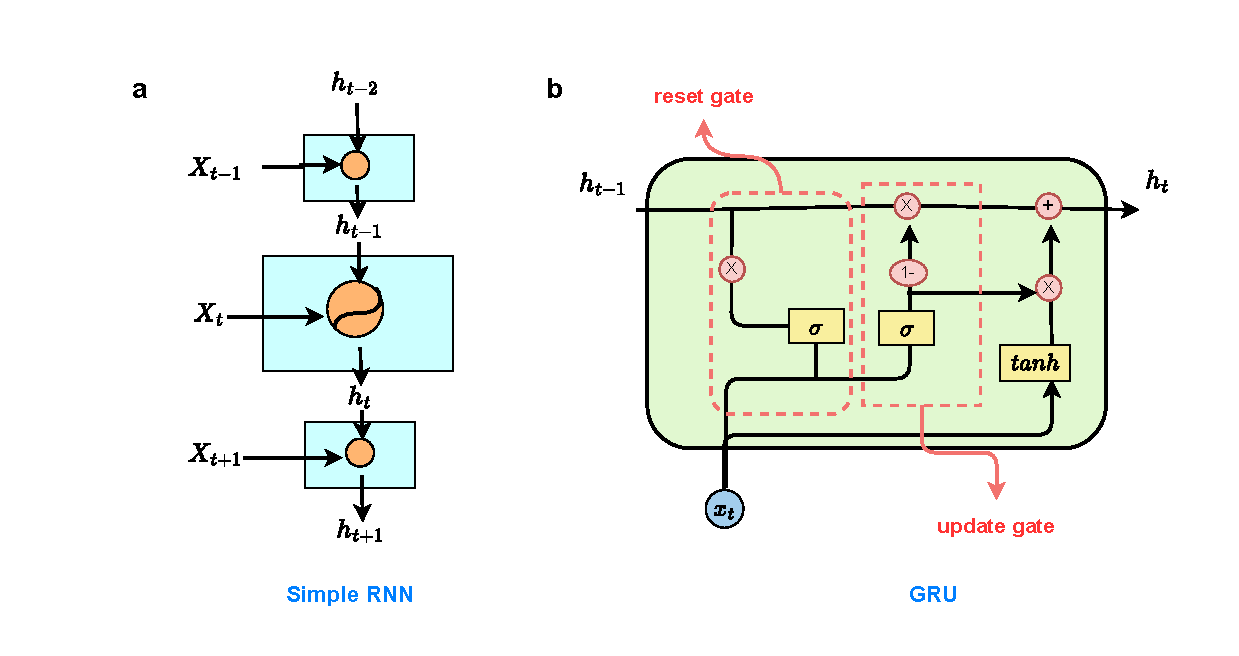
\includegraphics[width=0.9\textwidth]{Fig/rnn-gru.pdf}
  \FigureBicaption{\label{rnn_gru illustration}(a)RNN 示意图 ;(b)GRU 示意图}{Schematic illustration of (a) RNN and (b) GRU}
\end{figure}

候选隐藏状态决定了当前时间步的新信息,如公式\eqref{eq:gruhih}所示。
\begin{align}
  \tilde{\mathbf{h}}_t = \tanh(\mathbf{W}_h \mathbf{x}_t + \mathbf{U}_h (\mathbf{r}_t \odot \mathbf{h}_{t-1}) + \mathbf{b}_h) \label{eq:gruhih}
\end{align}
当前隐藏状态如公式\eqref{eq:gruhi}所示,这里的当前隐藏状态与上文LSTM的隐藏状态含义是一样的。
\begin{align}
  \mathbf{h}_t = (1 - \mathbf{z}_t) \odot \mathbf{h}_{t-1} + \mathbf{z}_t \odot \tilde{\mathbf{h}}_t \label{eq:gruhi}
\end{align}

GRU移除了单元状态的概念,直接从门控单元来计算隐藏状态,GRU 通过重置门和更新门的协同工作,实现了对信息流动的有效控制,使得网络能够在需要时记住长期依赖关系,同时减少梯度消失/爆炸的问题。GRU的结构比LSTM更简单,计算效率更高,因此在实践应用中广受欢迎。本文第三章使用GRU模型及其相关的复合模型进行流变学本构方程的预测建模。

GRU能够有效缓解梯度消失问题的关键在于其更新门机制。我们可以从梯度传播的角度进行分析。对于时间步$t$的隐藏状态$\mathbf{h}_t$,其关于时间步$t-1$的隐藏状态$\mathbf{h}_{t-1}$的梯度可以表示为:
\begin{align}
  \frac{\partial \mathbf{h}_t}{\partial \mathbf{h}_{t-1}} = \frac{\partial[(1 - \mathbf{z}_t) \odot \mathbf{h}_{t-1} + \mathbf{z}_t \odot \tilde{\mathbf{h}}_t]}{\partial \mathbf{h}_{t-1}} \label{eq:grugrad1}
\end{align}

展开上式,可得:
\begin{align}
  \frac{\partial \mathbf{h}_t}{\partial \mathbf{h}_{t-1}} & = (1 - \mathbf{z}_t) + \frac{\partial \mathbf{z}_t}{\partial \mathbf{h}_{t-1}} \odot (\tilde{\mathbf{h}}_t - \mathbf{h}_{t-1}) + \mathbf{z}_t \odot \frac{\partial \tilde{\mathbf{h}}_t}{\partial \mathbf{h}_{t-1}} \label{eq:grugrad2}
\end{align}

注意到第一项$(1 - \mathbf{z}_t)$是一个直接传递梯度的路径,这意味着当$\mathbf{z}_t$接近0时,前一时间步的隐藏状态几乎可以不经修改地直接传递到当前时间步。这种线性路径允许梯度在长时间步之间直接流动,有效避免了梯度消失问题。

与简单RNN相比,在RNN中,隐藏状态的梯度如公式\eqref{eq:rnngrad}所示:
\begin{align}
  \frac{\partial \mathbf{h}_t}{\partial \mathbf{h}_{t-1}} = \mathbf{W}_{hh} \cdot \sigma'(\mathbf{W}_{hh} \mathbf{h}_{t-1} + \mathbf{W}_{xh} \mathbf{x}_t + \mathbf{b}_h) \label{eq:rnngrad}
\end{align}

在RNN中,梯度必须经过非线性激活函数的导数$\sigma'$和权重矩阵$\mathbf{W}_{hh}$,这些连续的乘积会导致梯度消失。而在GRU中,由于更新门的存在,梯度可以通过$(1 - \mathbf{z}_t)$这一线性路径直接传递,从而在很大程度上缓解了梯度消失问题。

更新门$\mathbf{z}_t$实际上充当了一个自适应的开关,当需要保留长期记忆时,$\mathbf{z}_t$接近0,梯度可以几乎无损地传递;当需要关注当前输入时,$\mathbf{z}_t$接近1,网络会更多地考虑新信息。这种自适应的门控机制是GRU能够有效处理长期依赖关系的关键所在。

此外,重置门$\mathbf{r}_t$通过控制前一隐藏状态对候选隐藏状态的影响程度,使网络能够在需要时重置先前的记忆,这进一步增强了GRU捕获复杂时序模式的能力。综合来看,GRU通过其简化但高效的门控机制,在保持捕获长期依赖能力的同时,显著缓解了传统RNN中的梯度消失问题,使其成为时序建模的强大工具。
\subsection{其他时间序列算法}
在深度学习领域,针对时间序列数据的处理方法已呈现出多样化的趋势。除了传统的RNN及其变体,近年来研究人员提出多种新型网络架构,包括CNN、Transformer以及Mamba网络等,这些方法在时间序列分析中展现出显著的优势。

CNN最初是为图像处理任务设计的,但其在时间序列分析中的应用也取得了显著成效\cite{lecun1998gradient}。通过引入一维卷积操作,CNN能够有效地从时间序列数据中提取局部特征。由于卷积操作具有权值共享的特性,CNN在处理长序列数据时表现出较高的计算效率,并且能够有效规避传统RNN中常见的梯度消失或梯度爆炸问题。通过多层卷积结构的堆叠,CNN能够捕获更为复杂的时间依赖性,进而在语音识别、金融预测等实际应用中表现出优异的性能\cite{li2021survey}。

Transformer模型是近年来在自然语言处理领域取得突破性进展的架构,其核心在于自注意力机制\cite{Vaswanietal2017Attention}。与传统的RNN类模型不同,Transformer摒弃了序列顺序处理的限制,转而通过全局上下文信息建模序列中各元素之间的依赖关系。这种机制使得Transformer能够并行处理长序列数据,并捕获全局时序特征。在时间序列分析任务中,Transformer通过自注意力机制能够聚焦于序列中的关键时间点,从而有效建模时序依赖性和非线性关系。这一特性使其在机器翻译、语音识别等任务中超越了传统模型的表现。

Mamba网络是近年来提出的一种新型时间序列处理架构,专门针对复杂时间序列数据的高效建模而设计\cite{gu2024mamba}。与传统的RNN或CNN模型相比,Mamba网络通过引入多尺度时序建模策略,能够同时捕获时间序列中不同时间尺度的特征。这种多尺度建模方法不仅增强了模型的表达能力,还提升了其在处理多变且复杂时序数据时的鲁棒性。这一特性使其在金融市场分析、气象预测等领域展现出广阔的应用前景。

这些方法不仅拓展了时间序列建模的理论边界,也为实际应用提供了更为强大的工具。本文的研究工作是选择一种可以处理时间序列的算法来对数值模拟的流变学数据进行建模预测,样本量在万级,属于中小规模数据集,综合考虑算法时空间复杂度和训练成本,选择RNN中的GRU作为基础算法模型。未来针对更多流变学数据和复杂场景,可以进一步研究其他前沿模型的应用。
\section{物理信息神经网络}
\subsection{理论基础}
PINN是一种融合深度学习与物理原理的混合建模范式,最初设计用于解决偏微分方程\cite{raissiPhysicsinformedNeuralNetworks2019a}。与传统的纯数据驱动神经网络不同,PINN通过在训练过程中引入物理约束条件,使模型不仅能从数据中学习统计规律,还能满足底层物理定律,从而显著提高模型的泛化能力和预测精度。PINN的核心思想在于将物理定律(通常表现为偏微分方程)作为先验知识嵌入神经网络的损失函数中,通过同时最小化数据拟合误差和物理方程残差来训练模型。这种方法使得PINN在保持神经网络高度非线性表达能力的同时,确保模型预测结果符合物理定律,增强了模型的物理一致性和可解释性。
\begin{figure}[htbp]
  \centering
  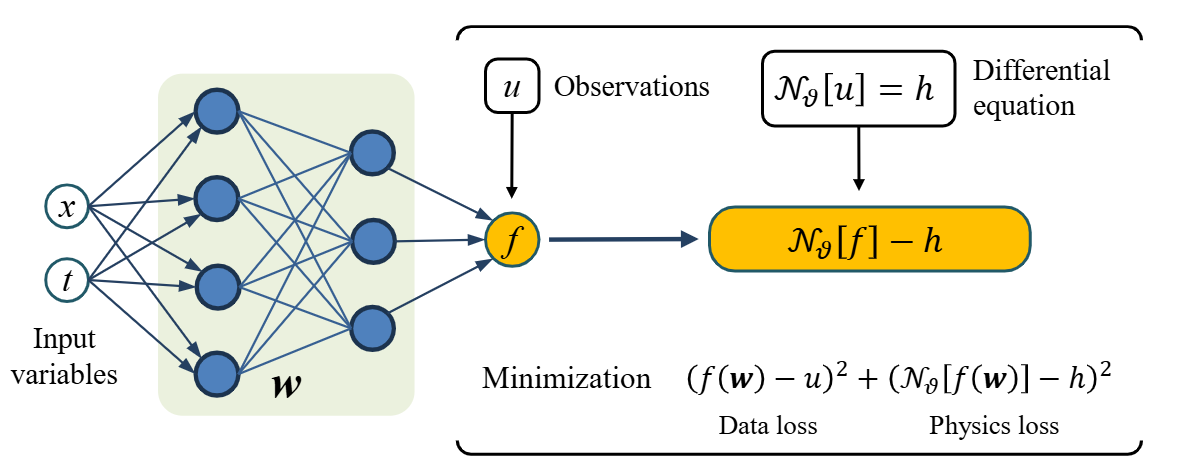
\includegraphics[width=0.8\textwidth]{Fig/pinn_logo.png}
  \FigureBicaption{\label{pinn illustration}PINN 示意图\cite{cuomoScientificMachineLearning2022}}{Schematic illustration of PINN\cite{cuomoScientificMachineLearning2022}}
\end{figure}
PINN的显著优势在于其能通过物理方程进行半监督或无监督训练,大幅降低对大规模标注数据的依赖。此外,PINN能确保模型预测符合物理定律,有效避免了纯数据驱动模型可能产生的物理不合理解。然而,PINN在处理高维复杂问题时仍面临训练收敛性和求解精度等挑战。
\subsection{损失函数构建}
PINN的核心在于其损失函数的精确构建。与传统前馈神经网络仅依赖数据损失$\mathcal{L}_{data}$不同,PINN的损失函数如公式\eqref{eq:pinnloss}所示,由数据损失和物理损失两部分组成,其中$\lambda$为平衡两种损失的权重系数。
\begin{align}
  \mathcal{L} = \mathcal{L}_{data} + \lambda\mathcal{L}_{physics} \label{eq:pinnloss}
\end{align}
数据损失用于量化神经网络预测值与实际观测数据之间的偏差,通常采用均方误差作为度量标准,如公式\eqref{eq:mse}所示。其中,$N_d$表示观测数据点的数量,$u(x_i, t_i)$表示神经网络在点$(x_i, t_i)$处的预测值,$u_i$为对应位置的真实观测值。
\begin{align}
  \mathcal{L}_{data} = \frac{1}{N_d} \sum_{i=1}^{N_d} \left( u(x_i, t_i) - u_i \right)^2 \label{eq:mse}
\end{align}
物理损失则确保神经网络的预测结果满足基本物理定律,通常通过计算物理方程的残差实现。以纳维-斯托克斯方程为例,其物理损失可表示为公式\eqref{eq:physicsloss}。本质上,物理损失反映了神经网络预测值在满足物理方程时的残差大小,残差越小,表明预测结果越符合物理规律。
\begin{align}
  \mathcal{L}_{physics} = \frac{1}{N_p} \sum_{j=1}^{N_p} \left( \frac{\partial u}{\partial t} + (\mathbf{u} \cdot \nabla) \mathbf{u} - \nu \nabla^2 \mathbf{u} - \nabla p + \mathbf{f} \right)^2 \bigg|_{(x_j, t_j)} \label{eq:physicsloss}
\end{align}
\subsection{前沿发展与优化方向}
公式\eqref{eq:pinnloss}中的权重参数$\lambda$控制物理损失与数据损失之间的相对重要性。当$\lambda$较大时,模型更倾向于满足物理约束;反之则更注重数据拟合。初期PINN研究常忽略此权重调节,使最终损失函数易受数据规模影响。特别是在多保真度建模中,若使用高保真数据计算数据损失,低保真数据计算物理残差,则当低保真数据量远大于高保真数据时,权重参数的精确设定变得尤为关键,以避免梯度消失或主导问题\cite{luDeepXDEDeepLearning2021}。

针对$\lambda$的优化,传统方法依赖经验调参,不仅缺乏理论依据,且耗时费力。近年来,自动化权重确定方法已成为研究热点。Farmer等人提出了一种经验性损失权重优化方法,用于PINN求解激光生物效应的1D热方程\cite{farmerEmpiricalLossWeight2024},通过自动归一化各损失项以保证平衡。Xiang等人开发了自适应损失平衡方法,基于高斯概率模型定义自适应损失函数\cite{xiangSelfadaptiveLossBalanced2022},该方法在每个训练周期中基于最大似然估计更新损失项权重,实验证明其在多种方程求解中优于传统PINN。Song等人提出基于损失注意力的PINN架构,为每个损失项配备独立的损失注意力网络\cite{songLossattentionalPhysicsinformedNeural2024},通过将训练点的平方误差动态加权,显著提高了预测精度和收敛速度。本研究借鉴并简化了Song的方案,实现了具有可学习权重的PINN框架。

在处理高维复杂偏微分方程时,PINN的计算效率仍是一项亟待解决的挑战。未来研究需重点提升计算性能以应对大规模问题\cite{Shah2024BenchmarkingQA-PINN}。此外,PINN在小样本学习方面的表现有待提高,需研发先进的自适应采样和数据增强技术,降低对大量训练数据的依赖。复杂物理约束的有效整合也是当前面临的难题,需开发更灵活强大的方法处理复杂方程和边界条件。在多物理场耦合问题中,PINN的应用范围仍较为局限\cite{Hillebrecht2022Certified,Haitsiukevich2023Improved},因此拓展PINN至多物理场耦合问题是解决复杂实际问题的关键研究方向。

\section{特征融合方法}
\subsection{简单特征融合}
特征融合是深度学习中一种重要的技术,旨在将来自不同来源或不同层次的特征进行组合,以创建一个捕获集体信息的统一表示。这种技术通过利用来自不同特征集的互补信息,能够显著增强模型的性能。

简单的特征融合方法包括Concat、Add和Hadamard Product等。其中,Concat是将两个特征向量拼接在一起,如公式\eqref{eq:concat},适用于需要保留两个特征向量的所有信息的场景。例如,在流体力学中,当需要同时考虑不同物理场(如速度场和压力场)或不同尺度的特征时,Concat 是一种合适的方法。Add是将两个特征向量逐元素相加,如公式\eqref{eq:add},适用于两个特征向量维度相同,且需要强调某些共同特征时。例如,需要将速度场的不同分量相加,可以突出重要的流动特征的时候,可以使用Add方法。Hadamard Product是将两个特征向量逐元素相乘,如公式\eqref{eq:hadamard}。当需要突出共同出现的特征并减弱不重要的特征时,Hadamard Product是一种合适的方法。例如,在流体力学中,如果需要将速度场和压力场的特征相乘,希望突出共同的流动特征时,在材料科学中,如果需要将材料编码和组分含量相乘,突出加权的含量特征时,都可以使用Hadamard Product。
\begin{align}
  \mathbf{v} & = [\mathbf{v}_1; \mathbf{v}_2] \label{eq:concat}          \\
  \mathbf{v} & = \mathbf{v}_1 + \mathbf{v}_2    \label{eq:add}           \\
  \mathbf{v} & = \mathbf{v}_1 \odot \mathbf{v}_2     \label{eq:hadamard}
\end{align}
\subsection{注意力特征融合}
深度学习中,注意力特征融合是一种重要的技术,它通过引入注意力机制来动态调整特征的权重,从而更好地融合特征\cite{dai2021attentional}。注意力特征融合的核心思想是利用注意力机制来捕获特征之间的关系,从而增强重要特征并减弱不重要的特征。注意力特征融合的数学公式如公式\eqref{eq:attentionsusion}所示,其中$\mathbf{v}_i$为特征向量,$\alpha_i$为注意力权重,$\mathbf{q}$为查询向量,用于计算注意力权重。
\begin{equation}
  \begin{aligned}
     & \mathbf{v} = \sum_{i=1}^{n} \alpha_i \mathbf{v}_i                                                 \\
     & \alpha_i = \frac{\exp(\mathbf{q}^T \mathbf{v}_i)}{\sum_{j=1}^{n} \exp(\mathbf{q}^T \mathbf{v}_j)}
  \end{aligned}   \label{eq:attentionsusion}
\end{equation}

在多尺度特征融合中,注意力机制的应用极大地提升了模型对不同尺度特征的动态权重调整能力,从而更有效地捕获全局和局部信息。这种方法在目标检测和图像分割等任务中表现出色,因为它能够更好地处理不同尺度的目标。例如,CM-UNet模型通过多尺度注意力聚合模块,在遥感图像语义分割任务中高效捕捉局部和全局信息,提升了特征表达能力\cite{Cui2023CMUnet}。

在实现注意力特征融合时,通常会使用注意力模块,如自注意力或交叉注意力。自注意力机制允许模型在同一个序列内部捕获特征之间的关系,而交叉注意力机制则允许模型在两个不同的序列之间捕获特征之间的关系。例如,交叉注意力可以用于将图像特征与文本特征进行融合,从而实现更准确的图像描述生成。在多模态学习中,交叉注意力机制通过在不同模块之间引入注意力机制,让信息交流更高效,也让模型在处理复杂任务时表现得更出色\cite{rong2023dynstatf}。

此外,注意力特征融合还可以与其他特征融合方法(如Concat和Add)结合使用。例如,在某些模型中,可以先使用Concat将不同来源的特征拼接在一起,然后使用注意力机制对拼接后的特征进行加权,从而进一步增强特征的表示能力。这种方法在多模态学习中特别有用,因为它可以有效地融合来自不同模态的特征。例如,多模态融合网络使用多头自注意力机制来最小化不同模态之间的噪声干扰,并利用局部区域特征表示之间的相关性来提取互补信息\cite{nagrani2021attention}。

总结注意力机制在多尺度特征融合和多模态学习中具有广泛的应用前景,能够显著提升模型的性能和泛化能力。通过合理设计和应用注意力模块,可以更好地捕获和融合不同尺度和模态的特征,从而在各种任务中取得更好的效果。而针对本文流变学的本构建模任务,由于制备参数(分子量、组分比例等)特征存在隐藏联系,但是特征本身非常稀疏,所以采取注意力特征融合的方法,期待显著提高模型的性能和泛化能力。
\section{生成式模型}
\subsection{变分自编码器}
生成式模型是一类能够学习数据生成过程的统计模型。它们通过建模数据的联合概率分布,能够生成与数据相似的新样本。与判别式模型(关注于建模条件概率分布)不同,生成式模型关注数据的整体结构和分配。

变分自编码器(Variational Autoencoder, VAE)是一种生成模型,结合了自编码器架构和变分推断方法。其核心思想是通过编码器将输入数据映射到潜在变量的分布参数(通常是均值和方差),然后通过解码器从这个分布中采样并重构输入数据。VAE的概念最早由Diederik提出。VAE的数学表达式如公式\eqref{eq:vae}所示。其中编码器将输入数据映射到潜在变量空间,解码器将潜在变量映射回原始输入空间。VAE的目标是最小化重构损失和变分下界的差异\cite{kingma2013auto}。
\begin{equation}
  \mathcal{L}(\theta_E, \theta_D) = \mathbb{E}_{q_{\theta_E}(z|x)} \left[ \log p_{\theta_D}(x|z) \right] - D_{KL}(q_{\theta_E}(z|x) \| p(z)) \label{eq:vae}
\end{equation}
重构损失$L_{rec} = \frac{1}{N} \sum_{i=1}^{N} \frac{1}{2} \| x_i - \hat{x}_i \|^2$用于衡量模型输出的重构精度,通常采用均方误差或交叉熵等损失函数,变分下界$L_{vae} = \mathbb{E}_{q_{\theta_E}(z|x)} \left[ \log p_{\theta_D}(x|z) \right] - D_{KL}(q_{\theta_E}(z|x) \| p(z))
$用于最大化潜在变量分布的重构似然。为了使 VAE 的训练过程可微分,引入了重参数化技巧。具体来说,假设潜在变量$z$服从均值为$\mu$、方差为$\sigma$的高斯分布,可以通过公式$z = \mu + \sigma \cdot \epsilon$从分布中采样,$\epsilon$是标准正态分布的随机变量。

VAE能够生成与训练数据类似的样本,例如人脸、文字等。在标签数据稀缺的情况下,VAE可以利用无标签数据学习数据的潜在结构,从而增强模型的泛化能力。凭借这一特性,VAE在图像生成、数据增强、无监督学习等多个领域展现出广泛的应用潜力,已成为生成模型领域的重要研究方向。
\subsection{条件变分自编码器}
条件变分自编码器CVAE的概念最早由Sohn等人提出\cite{SohnLee2015ConditionalVAE}。CVAE是VAE的扩展,它在VAE的基础之上引入了条件变量,使得生成的样本可以根据特定条件进行控制。CVAE 的核心思想是将条件变量$y$作为输入的一部分,与输入数据$x$一起编码到潜在变量$z$中,然后通过解码器生成样本。CVAE的目标是最大化条件似然$p(x|y) = \int p(x|z,y) p(z|y) dz$,损失函数公式为式\ref{eq:cvae}。
\begin{figure}[htbp]
  \centering
  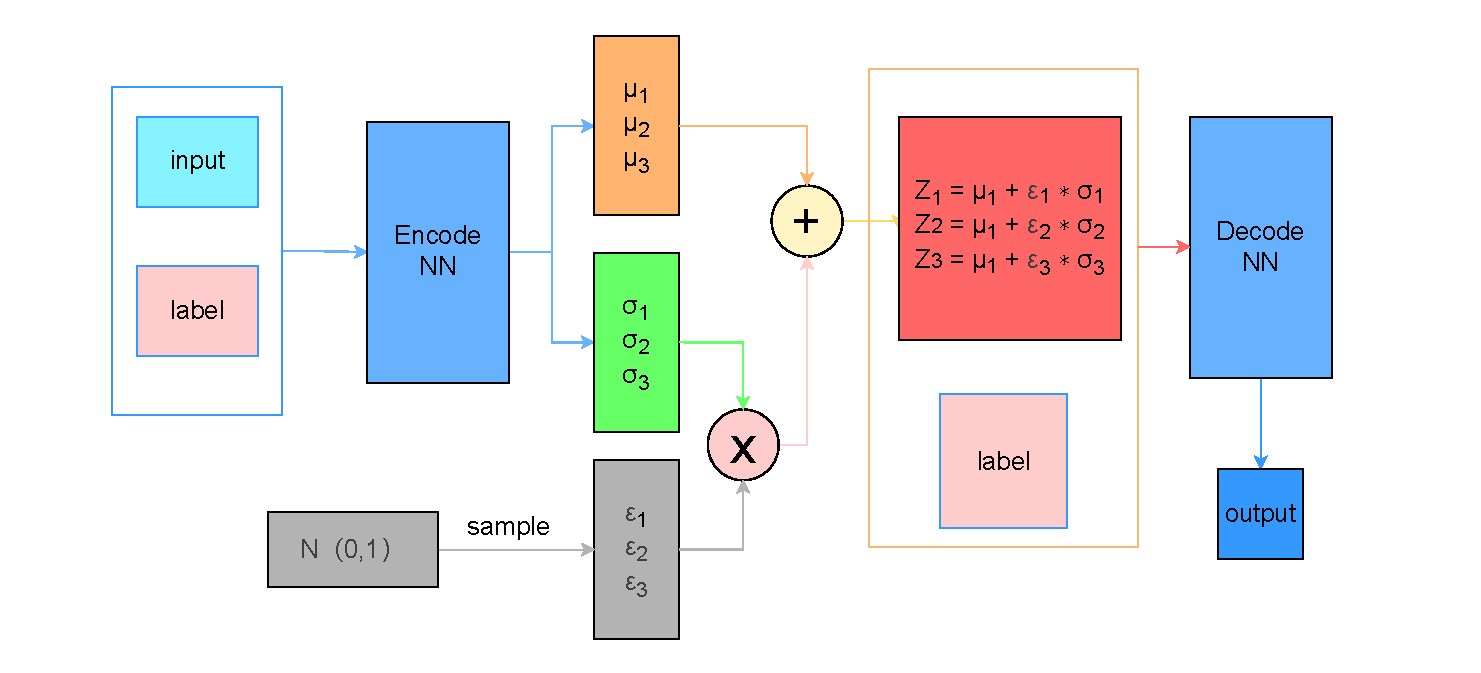
\includegraphics[width=0.8\textwidth]{Fig/CVAE示意图.drawio.pdf}
  \FigureBicaption{\label{cvae illustration}CVAE 示意图}{Schematic illustration of CVAE}
\end{figure}
\begin{equation}
  \mathcal{L}(\theta_E, \theta_D) = \mathbb{E}_{q_{\theta_E}(z|x,y)} \left[ \log p_{\theta_D}(x|z,y) \right] - D_{KL}(q_{\theta_E}(z|x,y) \| p(z|y))
  \label{eq:cvae}
\end{equation}
其中,第一项是重构损失,用于衡量模型输出与真实数据的差异;第二项是KL散度,用于衡量后验分布与先验分布之间的差异。通过最小化这一损失函数,CVAE能够学习到数据的生成分布,并生成与训练数据类似的样本。
CVAE引入条件变量$y$使得模型能够根据特定条件生成样本,这对于许多实际应用非常重要。例如,在图像生成任务中,条件变量可以控制生成图像的类别或属性。通过指定不同的条件变量,CVAE可以生成不同类别的图像,如不同类型的动物、不同的场景等。这使得CVAE在图像生成领域具有广泛的应用前景。

在自然语言处理任务中,条件变量可以控制生成文本的主题或风格。通过指定不同的条件变量,CVAE可以生成不同主题的文本,如新闻报道、故事、诗歌等。此外,条件变量还可以控制文本的风格,如正式、幽默、悲伤等。这使得 CVAE在自然语言生成领域具有重要的应用价值。

此外,CVAE 还可以在标签数据稀缺的情况下,利用无标签数据学习数据的潜在结构,从而增强模型的泛化能力。在实际应用中,标签数据往往非常稀缺,而无标签数据相对丰富。CVAE可以利用无标签数据学习数据的潜在结构,从而提高模型的性能。这使得CVAE在半监督学习和无监督学习中具有重要的应用价值。

在本文的工作中,我们希望通过已有的流变学性质参数,如特定频率下的储存模量($\mathrm{G^{\prime}}$)、损耗模量($\mathrm{G^{\prime\prime}}$)和损耗角正切(tan$\delta$)等,来预测特定的制备参数。CVAE能够将输入数据映射到高维潜在空间,并通过将流变学参数作为条件($y$)输入,生成特定的制备参数。

传统的深度神经网络,尤其是回归或分类网络通常直接进行输入到输出的映射,缺乏对潜在空间的建模,因此可能无法捕捉到数据背后复杂的分布。相比之下,CVAE作为生成模型,能够学习输入数据的潜在分布。它不仅依赖于输入数据的特征,还引入了条件信息,使得它能够在潜在空间中生成符合条件的参数,而不仅仅是进行简单的映射。

此外,CVAE通过变分推断捕获数据中的不确定性,能生成多个样本。对于制备参数,可能存在多个合理的组合或生成路径,CVAE通过潜在变量的不同采样来生成这些多样化的样本,从而增强了生成结果的多样性。而传统的DNN模型通常是确定性的,即给定相同的输入总是生成相同的输出,无法有效地表示这种不确定性。

最后,CVAE通过引入变分推断,平衡了重建误差和潜在变量的KL散度,从而在优化过程中不仅考虑了生成结果的质量,还保证了潜在空间的结构化。这使得CVAE能够生成接近原始数据的样本,并通过潜在空间的结构化生成有意义的样本。相比之下,DNN训练时通常只关注误差最小化,缺少对潜在空间结构的显式建模。
\subsection{其他生成式模型}
生成式模型是机器学习领域的重要研究方向,旨在学习数据的分布特征,从而生成与原始数据相似的新样本。除了VAE和CVAE之外,还有多种生成式模型在不同领域取得了显著成果。

自回归模型基于条件概率链式分解对数据进行建模,通过逐步生成数据单元完成整体构建\cite{bengio2003adaptive}。这类模型在密度估计方面展现出卓越性能,典型代表如PixelCNN和PixelSNAIL已成功应用于图像生成、语音合成等领域。然而其固有特性也带来若干限制:采样过程必须严格遵循序列生成路径,导致高维数据生成效率显著降低;同时模型强制要求将输入数据线性化为固定顺序,这在文本和音频等具有自然时序结构的模态中尚可适用,但对于图像等空间数据而言,最优排列方式的确定缺乏明确依据,且不同的顺序选择可能通过神经网络架构的归纳偏置对最终效果产生潜在影响\cite{bondtaylor2022deep}。

GAN是一种基于博弈论框架的生成模型,其核心由生成器与判别器构成动态博弈系统\cite{NIPS2014_5ca3e9b1}。生成器通过参数化映射函数将潜在空间向量转化为合成数据,旨在捕捉真实数据分布的统计特性;判别器则作为二元分类器,通过迭代优化提升对真实数据与生成数据的鉴别能力。二者在对抗性训练过程中形成“最小---最大”博弈关系:生成器试图生成高度逼近的样本来欺骗判别器,而判别器则持续升级其辨别能力以识别生成样本的统计缺陷,最终推动系统向纳什均衡收敛。相较于传统生成模型,GAN的突出优势在于其能通过对抗机制隐式学习复杂数据分布,生成具有高度视觉保真度的样本(如图像、视频)\cite{Goodfellow2020Generative}。

扩散模型是新一代生成式人工智能的核心范式,其创新性地将数据生成过程建模为物理学启发的渐进式去噪机制\cite{ho2020denoising}。该模型通过构建马尔可夫链,系统性地模拟两个互逆过程:前向扩散阶段将原始数据通过逐步添加高斯噪声退化为随机噪声,反向生成阶段则通过参数化的神经网络学习逆向扩散轨迹,从纯噪声出发通过连续的去噪操作重建出目标数据分布。这种基于随机微分方程或概率流常微分方程的数学框架,使得模型能够通过变分推断精确优化对数似然下界\cite{song2020score}。相较于GAN,其生成过程具有可解释的物理意义,通过调节去噪步长可实现生成质量与速度的灵活平衡;无需对抗训练避免了模式崩溃风险,确保生成样本的多样性,且理论框架的严密性支持精确的概率密度估计\cite{Cao2024Survey}。
\section{本章小结}
本章系统阐述了深度学习算法在流变学本构建模中的理论基础与应用框架,为后续研究奠定了方法论基础。

首先,针对时序建模技术,本章详细分析了循环神经网络及其变体(尤其是GRU)的核心机制及优势,阐明了其在捕捉流变材料时间依赖性行为方面的适用性,特别是在处理应力松弛等记忆效应现象时的优越性。这些理论为第三章中基于GRU的本构模型识别与预测提供了算法支撑,使我们能够有效处理流变学中的时序依赖性问题。

之后,本章详细介绍了PINN的发展历史、基本数学原理和前沿的优化方向,为物理信息神经网络在流变学中的应用奠定了基础。这一理论框架贯穿第三章与第四章的研究,分别在本构关系预测与材料设计反问题中发挥核心作用,实现了数据与物理规律的有机结合。

在特征融合方法方面,本章介绍了简单特征拼接和多尺度特征融合的方法以及相关的数学原理,并说明了本文后续实验中选取的特征融合方法的依据。这些方法将在第四章中用于整合不同来源和尺度的特征,特别是在处理制备参数与流变性能之间复杂关联时发挥重要作用。

对于生成式模型,本章系统介绍了VAE及其条件变体CVAE的理论框架,分析了它们在处理流变学参数与制备参数之间映射关系时的优势,尤其是在捕捉多参数组合可能性方面的潜力。这些生成模型理论将在第四章中应用于材料设计的反向问题求解,为从期望性能反推制备参数提供了新途径。

通过构建这一算法体系,本文为突破传统流变学本构方程的表达限制,发展数据驱动与物理约束相结合的智能建模方法提供了理论支撑和技术路径。本章介绍的各类算法将在后续章节中结合,形成完整的技术链条。